\begin{table}[h!]
    \centering
    \begin{tabular}{|c|c|c|c|}
        \hline
        \textbf{Anzahl Hinweise} & \textbf{Anzahl true} & \textbf{Anzahl total} & \textbf{Wahrscheinlichkeit} \\
        \hline
        21 & 0     & 3     & 0.00\% \\
        22 & 4     & 147   & 2.72\% \\
        23 & 786   & 1829  & 42.97\% \\
        24 & 10883 & 11879 & 91.62\% \\
        25 & 30508 & 30638 & 99.58\% \\
        26 & 33783 & 33786 & 99.99\% \\
        27 & 16948 & 16948 & 100.00\% \\
        28 & 4235  & 4235  & 100.00\% \\
        29 & 513   & 513   & 100.00\% \\
        30 & 21    & 21    & 100.00\% \\
        31 & 1     & 1     & 100.00\% \\
        \hline
    \end{tabular}
    \caption{Übersicht: Anzahl Hinweise, Anzahl true, Anzahl total und Wahrscheinlichkeit (in Prozent) pro Wert}
\end{table}

\begin{figure}[h!]
    \centering
    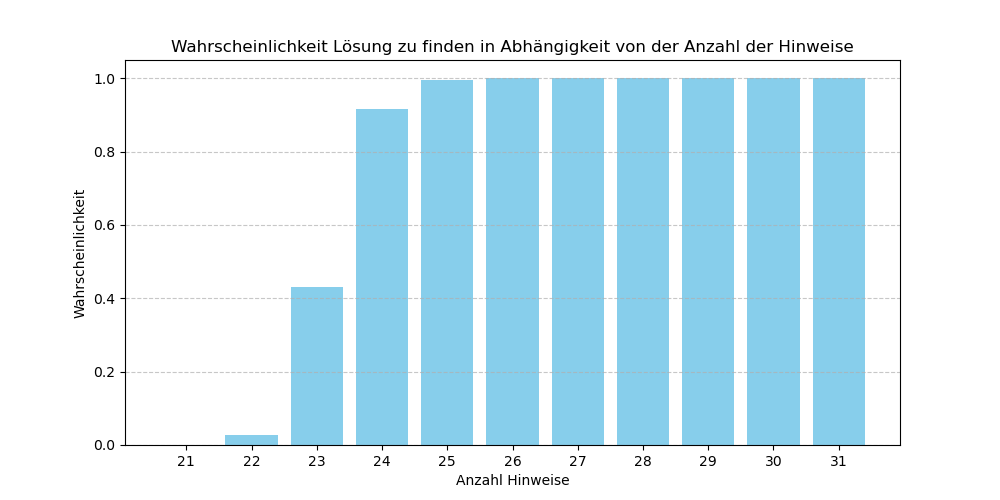
\includegraphics[width=0.8\textwidth]{Pictures/wahrscheinlichkeiten}
    \caption{Wahrscheinlichkeit, dass ein Sudoku mit einer bestimmten Anzahl an Hinweisen eindeutig lösbar ist}
    \label{fig:wahrscheinlichkeiten}

\end{figure}

\begin{figure}[h!]
    \centering
    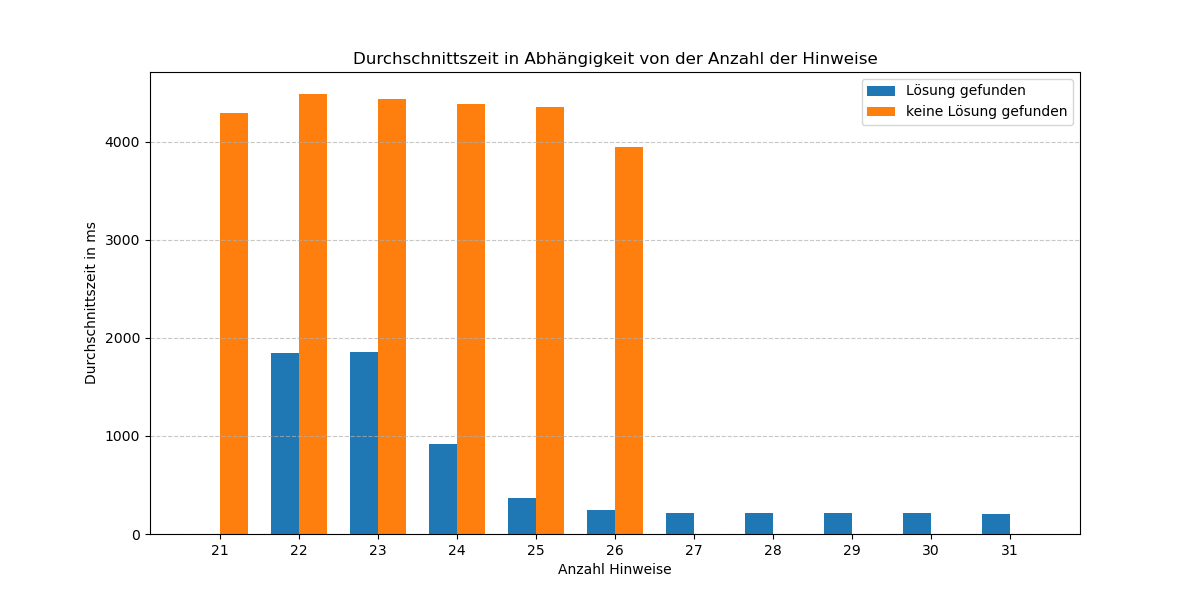
\includegraphics[width=0.8\textwidth]{Pictures/zeiten}
    \caption{Wahrscheinlichkeit, dass ein Sudoku mit einer bestimmten Anzahl an Hinweisen eindeutig lösbar ist}
    \label{fig:zeiten}
\end{figure}